\chapter{Resultados Obtidos}
\label{cap:impl}

Para realização dos testes, foram
selecionados 6 tópicos distribuídos em duas categorias diferentes, que são:
comentários políticos e comentários sobre filmes. Optou-se pela escolha de duas
categorias distintas com o objetivo de avaliar a assertividade do método
desenvolvido em diferentes contextos. Como a validação dos resultados é efetuada
de forma manual, não foi possível efetuar a análise sobre mais tópicos ou
categorias.

\section{Comentários Políticos}

De forma a realizar testes sobre um contexto de comentários políticos, foi
executado o método de Propagação Dupla, através dos próprios comentários e então
selecionada a palavra \textit{``Trump''}, como a palavra alvo para
restrição na análise de comentários. Desta forma, os tópicos selecionados para
essa análise estão listados abaixo. Esses foram descritos na seção
\ref{sec:textos}.

\begin{itemize}
  \item
  \textit{Donald Trump to strip all funding from State Dept team promoting
  women's rights around the world - Leaked plan comes as First Daughter Ivanka
  defends her father's record with women}.  
  \item
  \textit{Sweden asks the U.S. to explain Trump comment on
  Sweden}.
  
  \item\textit{“Canada will welcome you,” Trudeau invites refugees as Trump bans
  them}.
\end{itemize}

 
\begin{figure}[!htbp]
\centering
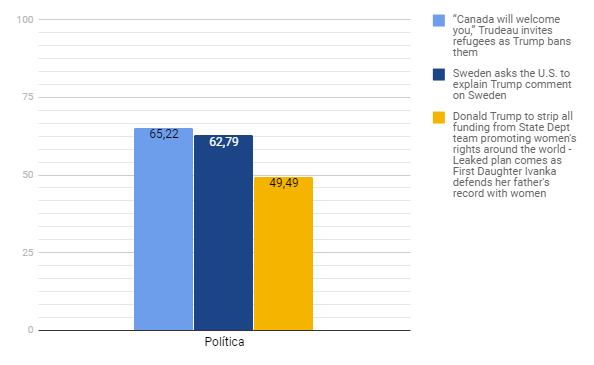
\includegraphics[height=250px]{imagens/politica1.png}
\caption{Assertividade da ferramenta desenvolvida com relação a comentários de
política.}
\label{fig:pol1}
\end{figure}

Na Figura \ref{fig:pol1}, tem-se os resultados obtidos. Observa-se que
a assertividade foi próxima aos valores obtidos por Hutto e Gilbert
\cite{conf/icwsm/HuttoG14} para avaliações de produtos da Amazon e para
editoriais do New York Times. Porém, os valores foram inferiores aos obtidos na
avaliação de \textit{tweets}. A partir desse resultado, acredita-se que a
assertividade da ferramenta está relacionada com o contexto de utilização
desta, demonstrado pela diferença na assertividade entre os tópicos. De forma a
avaliar se os resultados foram ocasionados pela diferença de contexto ou por seus corpos de texto terem diferentes tamanhos, foi também conduzida uma análise separando todos os comentários de política em três categorias, comentários com 144 caracteres ou
menos, similares a \textit{``tweets''}, tópicos com menos de 1000 caracteres e
tópicos com 1000 caracteres ou mais.

\newpage
 
\begin{figure}[!htbp]
\centering
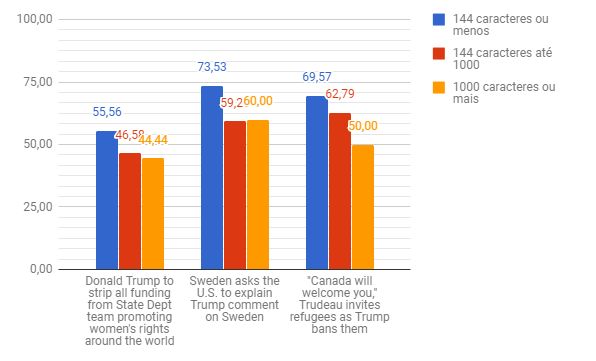
\includegraphics[height=250px]{imagens/politica2.png}
\caption{Assertividade da ferramenta desenvolvida com relação a comentários de
política por tamanho.}
\label{fig:pol2}
\end{figure}

Na Figura \ref{fig:pol2} tem-se os resultados obtidos através da
análise através da quantidade de caracteres. Pode-se observar que o método
apresenta uma diminuição na sua assertividade com o aumento do texto. 

\section{Comentários sobre Filmes}

Os mesmos testes foram realizados utilizando a palavra \textit{``movie''} como
alvo, em tópicos de cinema. O método \ac{VADER}, foi utilizado usando o método
de Propagação Dupla, sendo que os textos selecionados para a expansão e, para a
posterior análise foram obtidos dos comentários dos tópicos:

\begin{itemize}
  \item
  \textit{Official Discussion - mother! [SPOILERS]}: esse tópico contém 5297
  comentários e encontra-se disponível em
  \textit{\url{https://www.reddit.com/r/movies/comments/706y1p/official_discussion_mother_spoilers/}}
  e apresenta a avaliação do filme \textit{``Mother!''}.
  \item
  \textit{Official Discussion: Gerald's Game [SPOILERS]}: esse tópico contém 892
  comentários e
  encontra-se disponível em
  \textit{\url{https://www.reddit.com/r/movies/comments/73g2fx/official_discussion_geralds_game_spoilers/}}
  e apresenta a avaliação do filme \textit{``Gerald's Game''}.
    \item
  \textit{Official Discussion: The Mummy (2017) [SPOILERS]}: esse tópico contém
  1333 comentários e
  encontra-se disponível em
  \textit{\url{https://www.reddit.com/r/movies/comments/6g5lmo/official_discussion_the_mummy_2017_spoilers/}}
  e apresenta a avaliação do filme \textit{``The Mummy''}.
  
\end{itemize}


Na Figura \ref{fig:fil1} tem-se os resultados obtidos. Observa-se que a
assertividade também se mostra próxima aos valores obtidos por Hutto e Gilbert
\cite{conf/icwsm/HuttoG14}, porém acima dos valores apresentados para
comentários de política. Acredita-se que isso é causado pois os
tópicos de discussão de filmes encorajam o leitor a avaliar o filme que está sendo discutido apresentando uma enquete em seu corpo, enquanto
os comentários sobre política apresentam no conteúdo de seu tópico somente um
\textit{link} direto para a notícia original. 


\newpage 


\begin{figure}[!htbp]
\centering
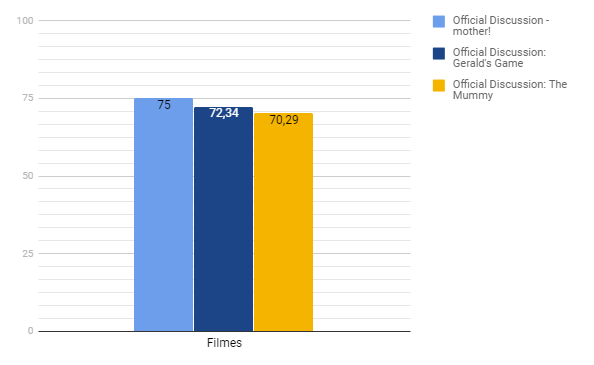
\includegraphics[height=250px]{imagens/filmes1.png}
\caption{Assertividade da ferramenta desenvolvida com relação a comentários de
filmes.}
\label{fig:fil1}
\end{figure}


Posteriormente, foi conduzida uma análise separando
todos os comentários de filmes em três categorias de acordo com o tamanho do
texto: comentários com 144 caracteres ou menos (similares a
\textit{``tweets''}), comentários com menos de 1000 caracteres e comentários com
1000 caracteres ou mais. Na Figura \ref{fig:fil2} tem-se os resultados obtidos através da
análise através da quantidade de caracteres. De forma similar aos comentários
de política, o método apresenta uma diminuição na sua assertividade com o
aumento do texto.

\begin{figure}[!htbp]
\centering
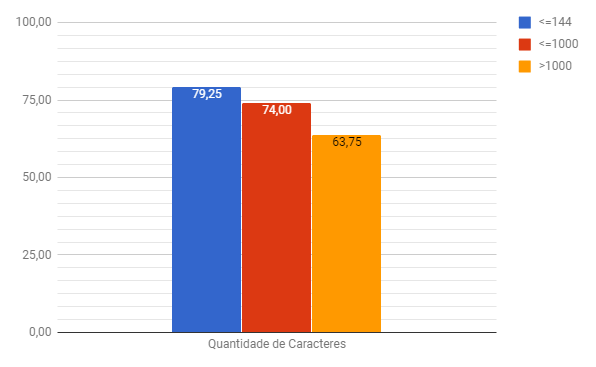
\includegraphics[height=225px]{imagens/filmes2.png}
\caption{Assertividade da ferramenta desenvolvida com relação a comentários de
filmes por tamanho.}
\label{fig:fil2}
\end{figure}

Através dos resultados
apresentados anteriormente, pode-se verificar que a ferramenta apresentou maior
assertividade ao análisar comentários de filmes (Figura \ref{fig:fil1}) do
que comentários políticos (Figura \ref{fig:pol1}).
Neste contexto, o resultado se mostrou similar ao apresentado por Pålsson e
Szerszen de 72,3\% \cite{SentimentinSocialMedia}.

Já com relação aos tópicos relacionados a política, a ferramenta
apresentou uma baixa assertividade, chegando a apresentar assertividade similar
a uma classificação realizada de forma aleatória, o que naturalmente iria
classificar os comentários com 50\% de acerto eventualmente.

Destaca-se que nos tópicos relacionados com
política não é pedido que o autor do comentário expresse sua opinião sobre o
que estamos querendo avaliar. Desta forma, o \ac{VADER} acaba atribuindo
sentimentos inexistentes ou com sua polaridade errada em determinadas frases,
como por exemplo, \textit{``\ldots What if he is just like trump and trump's
useless father\ldots``}. 

Neste caso, o dicionário irá avaliar de forma positiva o
comentário pois esse apresenta a palavra \textit{``like''}, que quando utilizada
com o significado de \textit{``gostar''} apresenta um sentimento positivo.
Porém, a palavra \textit{``like''} neste caso está sendo utilizada como
comparação.

Pode-se verificar que o método apresenta uma diminuição na sua assertividade
com o aumento do texto. Essa tendência é observada nos
trabalhos de Hutto e Gilbert \cite{conf/icwsm/HuttoG14} onde \textit{``tweets''}
analisados apresentaram maior assertividade do que editorias do \textit{New
York Times} e avaliações de produto da \textit{Amazon}.
